%!TEX root = ../thesis.tex
\documentclass[..thesis.tex]{subfiles}

\begin{document}
Profiling is an activity which aims to identify performance issues in an observable program. This task often relies of specific tools called profilers for extracting information from the program's execution. The output of the profiler helps to identify and locate the methods that have the largest effect on the program's execution time. Such methods are usually worth investigating as they affect the application's performance the most. \cite{mytkowicz_evaluating_2010}

Sampling profilers are a type of profiles which gather call traces from the observable program at varying intervals. A sample in the form of a call trace is a representation of a single thread's state at a particular moment in time. A simple call trace of a thread can be observed in listing ~\ref{lst:stack_trace}. 

\begin{lstlisting}[style=def,label={lst:stack_trace}, caption={Call trace of a thread}]
"main" #1 prio=5 os_prio=0 tid=0x00007feccc224000 nid=0x1f2c 
runnable [0x00007fecd5660000]
   java.lang.Thread.State: RUNNABLE
	    at ee.ut.SimpleBenchmark.methodA(SimpleBenchmark.java:28)
    	at ee.ut.SimpleBenchmark.doWork(SimpleBenchmark.java:22)
	    at ee.ut.SimpleBenchmark.main(SimpleBenchmark.java:11)
\end{lstlisting}

Gathered samples can then be aggregated and grouped based on their occurrence.
Distribution of the gathered samples highlights the hotspots in the observable program. Higher frequency of a call trace suggests that more program's execution time was spent in that particular state. 

Figure ~\ref{fig:samplingProf} on page ~\pageref{fig:samplingProf} helps to visualize the performance implications of the frequency of the gathered samples. The visualization was created by a tool called Flamegraphs which provides means to generate a comprehensive and intuitive visualization of the gathered call trace samples. \cite{gregg_flame} Visualization tools are necessary to produce meaningful representations of the collected data as unprocessed call trace samples \textit{per se} are not informative without the context of other samples' frequency.

\begin{figure}[H]
\includegraphics[scale=0.4]{equalsample.png}
\caption{Visualization of sampling profiling output}
\label{fig:samplingProf}
\end{figure}

The samples of the visualization in figure ~\ref{fig:samplingProf} were gathered from a simple program that executed two identical methods, \texttt{methodA} and \texttt{methodB}, alternately. During its execution $481$ usable samples were collected. $198$ of those samples contained \texttt{methodA} in its top call frame and $194$ contained \texttt{methodB} in its top frame.

Although sampling profiling does not provide precise metrics for each method's execution time, it can provide a general overview to visualize the time spent in the profileable application's context. Such information is often sufficient to make actionable optimizations in the observable application.

\subsection{Importance of samples' quantity}

For sampling profilers, the result is a statistical approximation of the program's performance. Thus, having more samples will provide a more accurate approximation. 

Figure ~\ref{fig:lowSampleCount} on page ~\pageref{fig:lowSampleCount} illustrates the problem which is caused by the low sampling interval. Suppose that the figure ~\ref{fig:lowSampleCount} resembles a program's execution in which the horizontal axis represents the current program's call trace state in that particular moment in time. It can be observed that the amount of time spent in method Y is significantly larger than the amount of time that was spent in methods X and Z. Suppose that the sampling profiler obtains a sample at each dotted vertical line. Such profiling results would represent each method X, Y and Z with a single sample. This implies that all the methods spent roughly the same amount of time during the execution of the program. The result is inaccurate as the visualization clearly shows that method Y spent roughly 4 times more time than it was spent for executing methods X and Z.

\begin{figure}[H]
\centering
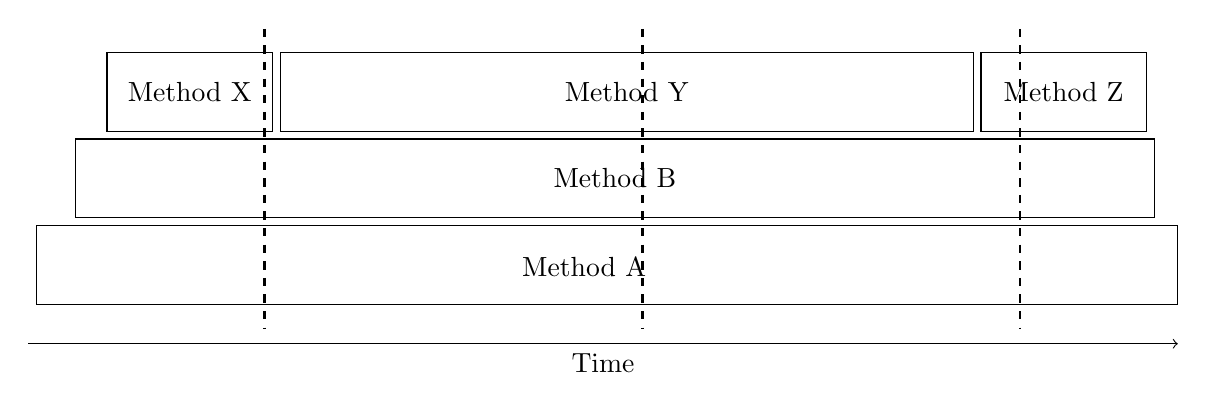
\begin{tikzpicture}
% Call stack rectangles
\draw (0,0) rectangle (14.5,1) node[pos=.48] {Method A};
\draw (0.5,1.1) rectangle (14.2,2.1) node[pos=.5] {Method B};

\draw (0.9,2.2) rectangle (3,3.2) node[pos=.5] {Method X};
\draw (3.1,2.2) rectangle (11.9,3.2) node[pos=.5] {Method Y};
\draw (12.0,2.2) rectangle (14.1,3.2) node[pos=.5] {Method Z};

% x-axis time arrow below
\draw[->] (-0.1,-0.5) -- (14.5, -0.5) node[below, pos=.5] {Time};

% samples
\draw[dashed, thick] (2.9,3.5) -- (2.9,-0.3);
\draw[dashed, thick] (7.7,3.5) -- (7.7,-0.3);
\draw[dashed, thick] (12.5,3.5) -- (12.5,-0.3);

\end{tikzpicture}
\caption{Scenario with low sampling interval}
\label{fig:lowSampleCount}
\end{figure}

Increasing the sampling interval would improve the situation as demonstrated on figure ~\ref{fig:highSampleCount} on page ~\pageref{fig:highSampleCount}. Upon profiling with a four times higher sampling interval, it becomes apparent that method Y call trace samples have been proportionally represented in the total call trace samples.

\begin{figure}[H]
\centering
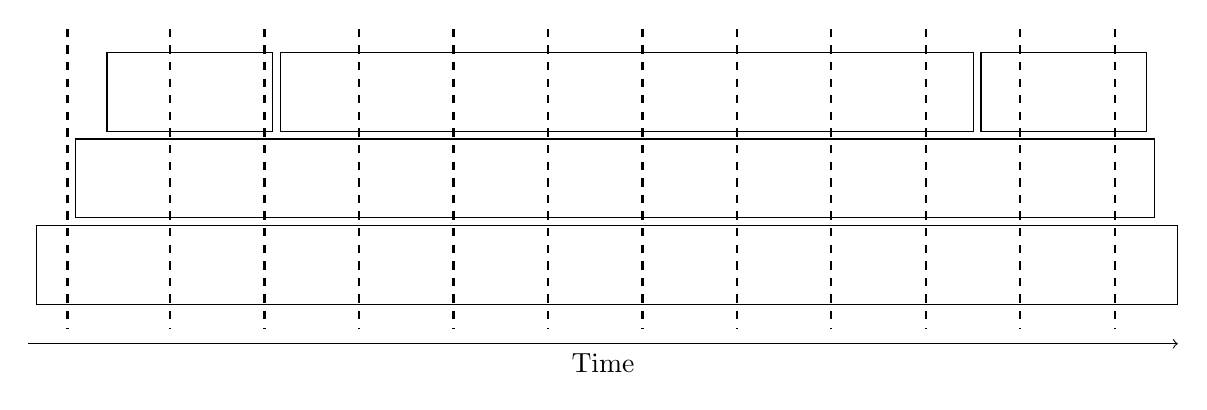
\begin{tikzpicture}
% Call stack rectangles
\draw (0,0) rectangle (14.5,1) node[pos=.48] {};
\draw (0.5,1.1) rectangle (14.2,2.1) node[pos=.5] {};

\draw (0.9,2.2) rectangle (3,3.2) node[pos=.5] {};
\draw (3.1,2.2) rectangle (11.9,3.2) node[pos=.5] {};
\draw (12.0,2.2) rectangle (14.1,3.2) node[pos=.5] {};

% x-axis time arrow below
\draw[->] (-0.1,-0.5) -- (14.5, -0.5) node[below, pos=.5] {Time};

% samples
\draw[dashed, thick] (0.4,3.5) -- (0.4,-0.3);
\draw[dashed, thick] (1.7,3.5) -- (1.7,-0.3);

\draw[dashed, thick] (2.9,3.5) -- (2.9,-0.3);
\draw[dashed, thick] (4.1,3.5) -- (4.1,-0.3);
\draw[dashed, thick] (5.3,3.5) -- (5.3,-0.3);
\draw[dashed, thick] (6.5,3.5) -- (6.5,-0.3);
\draw[dashed, thick] (7.7,3.5) -- (7.7,-0.3);
\draw[dashed, thick] (8.9,3.5) -- (8.9,-0.3);
\draw[dashed, thick] (10.1,3.5) -- (10.1,-0.3);
\draw[dashed, thick] (11.3,3.5) -- (11.3,-0.3);

\draw[dashed, thick] (12.5,3.5) -- (12.5,-0.3);
\draw[dashed, thick] (13.7,3.5) -- (13.7,-0.3);

\end{tikzpicture}
\caption{Scenario with sufficient sampling interval}
\label{fig:highSampleCount}
\end{figure}

\subsection{Sampling profiling challenges}
There are multiple problems that the implementations of the sampling profilers could experience that could potentially cause the results to be skewed.
\subsubsection{Periodicity bias}
This problem occurs when the sampling interval catches on to some program's routine which executions match the sampling interval. Figure ~\ref{fig:periodicityBias} on page ~\pageref{fig:periodicityBias} illustrates the issue behing the bias. Suppose that the observable program runs \texttt{Method X} and \texttt{Method Y} alternatingly for some constant time period. If the dotted lines are the marks for the call trace samples taken during profiling, the results would be skewed as not a single sample represents \texttt{Method Y} in the results. 

\begin{figure}[H]
\centering
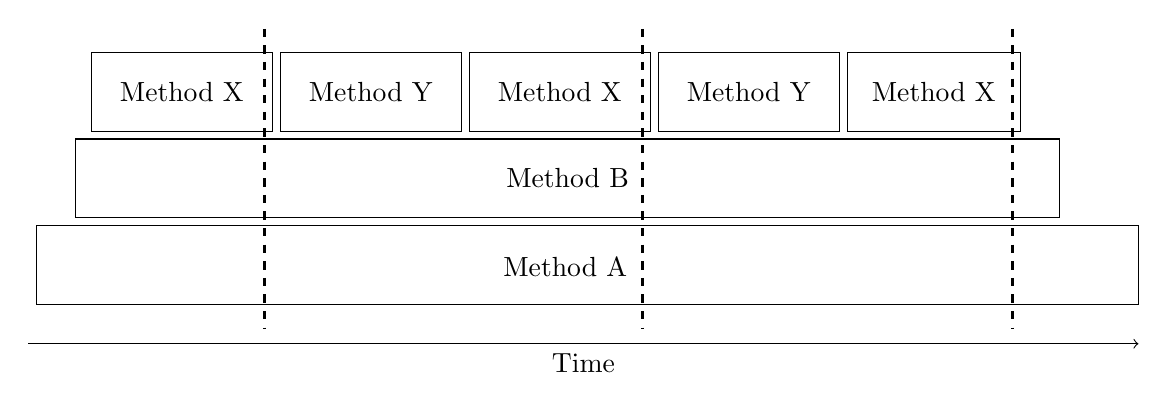
\begin{tikzpicture}
% Call stack rectangles
\draw (0,0) rectangle (14,1) node[pos=.48] {Method A};
\draw (0.5,1.1) rectangle (13,2.1) node[pos=.5] {Method B};
\draw (0.7,2.2) rectangle (3,3.2) node[pos=.5] {Method X};
\draw (3.1,2.2) rectangle (5.4,3.2) node[pos=.5] {Method Y};
\draw (5.5,2.2) rectangle (7.8,3.2) node[pos=.5] {Method X};
\draw (7.9,2.2) rectangle (10.2,3.2) node[pos=.5] {Method Y};
\draw (10.3,2.2) rectangle (12.5,3.2) node[pos=.5] {Method X};

% x-axis time arrow below
\draw[->] (-0.1,-0.5) -- (14, -0.5) node[below, pos=.5] {Time};

% samples
\draw[dashed, thick] (2.9,3.5) -- (2.9,-0.3);
\draw[dashed, thick] (7.7,3.5) -- (7.7,-0.3);
\draw[dashed, thick] (12.4,3.5) -- (12.4,-0.3);

\end{tikzpicture}
\caption{Illustration of periodicity bias}
\label{fig:periodicityBias}
\end{figure}

%Real life example can be observed on the figure ~\ref{fig:samplingProf} on page ~\pageref{fig:samplingProf}. The sample application called two identical methods alternatingly after a constant interval or $4$ milliseconds without any mechanism to combat this periodicity bias. On the output graph, it can be observed that the \texttt{methodA} was present in a larger amount of samples than \texttt{methodB}. In reality, it would be expected for \texttt{methodA} and \texttt{methodB} to have approximately the same number of call trace samples representing them.

Possible way to tackle this problem would be to randomize the sampling interval by having a random number of time units offseting the sampling interval. Increasing sample gathering frequency will also help to alleviate this problem.

\subsubsection{Safepoint bias}

Sampling profiling assumes that samples are gathered randomly as bias in the samples could potentially yield inaccurate results. When gathering samples from a program running on the Java Virtual Machine (JVM), one must take \textit{safepoints} into consideration. 

Safepoints in the Java Virtual Machine are defined as points during the program's execution during which all of the threads are in a consistent and well known state. Safepoints are necessary for various Java Virtual Machine's operations such as the garbage collection, method deoptimization and class redefinition.\cite{hotspot_glossary} It has been shown that most of the existing Java profilers require the Java Virtual Machine to be stopped on a safepoint in order to obtain the call trace sample from the profileable thread.\cite{wakart_psychosomatic_2016} However, this mechanism also casts a shadow on the profling results as this implies that the samples are not acquired randomly but rather require the Java Virtual Machine to be in a specific state. \cite{mytkowicz_evaluating_2010}

The execution of the code sample in listing ~\ref{lst:safepoint} illustrates this issue well. 
\TODO{Verify that this code snippet is completely rendered on the same page in the final version}


\begin{lstlisting}[language=java,style=def,label={lst:safepoint}, caption={Counted loops do not contain safepoints}]
int k = 0;
for (int i = 0; i < Integer.MAX_VALUE; i++) {
	for (int j = 0; j < 2; j++) {
    	k++;
    	if ((k % 2) == 1) k++;
	}
}
\end{lstlisting}
As various Java Virtual Machine routines are nondeterministic, it is impossible to predict when does the Java Virtual Machine signal its threads to be stopped on a safepoint. However, if such request should occur in the middle of the counted loop's execution in listing ~\ref{lst:safepoint}, the thread executing the loop's instructions will not stop until the loop has finished. Thus, if an ordinary sampling profiler signals the thread for a call trace sample, it is delayed until the thread executing the loop's instructions finishes its task. \cite{wakart_psychosomatic_2015}

To measure the actual time that is spent waiting for the Java Virtual Machine to stop all its threads on a safepoint, \texttt{-XX:+PrintGCApplicationStoppedTime} flag can be used to measure this metric. This flag outputs the time it takes for the Java Virtual Machine to stop all threads in order to execute its subroutine and the time that this operation took in total. Due to nondeterminicity, the sample code in listing ~\ref{lst:safepoint} was executed $100$ times. The worst case among $100$ program runtimes recorded a Java Virtual Machine operation that took $7.517$ seconds and $99.999\%$ of that time was spent on reaching a safepoint. It is worth mentioning that this operation took $65\%$ of the whole program's execution time.

Although the provided example is rather artificial and such occurrences in real life programs are rare, it clearly points out the bias that the safepoints potentially introduce. Such bias during obtaining the call trace clearly contradicts the randomness prerequisite for sampling profiling. Despite the presence of safepoint bias, such profiler can still produce actionable profiling results but lessen the accuracy when high detail granularity of the results is important.


%\TODO{Ideas to expand on:}
%\TODO{Should I explain the implementation side of the safepoints more in-depth?}
%Safepoints are not precisely documented in the language specifications as they are implementation details of the JVM and each JVM implementation may interpret safepoints differently but they generally work in a similar manner.

%JVM raises a flag to notify threads to stop on safepoint and then waits the threads to stop on a safepoint. Thread polls for safepoint flag after every 2 bytecode instructions (when in interpreter), end of non-counted loop, method exit, JNI call exit(C1/C2 compiled code)

\subsubsection{Observer effect}

Attaching a profiler to the observable application does alter the way how the application would normally execute. The \textit{observer effect} describes how a presence of a profiler can change the profiling outcome.
 
Firstly, a profiler does introduce some performance overhead due to its nature. Profilers do need to execute additional instructions for gathering information from the observable application. To have meaningful profiling results, this overhead must not affect the application's performance by a large extent.

The presence of a profiler could also change the way how the Java Virtual Machine does its optimizations. This factor affects sampling profilers as well but it is especially relevant for tracing profilers as they rely on bytecode instrumentation which directly affects the way how the Java Virtual Machine performs its optimizations. Some optimizations might not be possible due to the added bytecode instructions added by the tracing profiler. \cite{mytkowicz_evaluating_2010} 

\TODO{Perhaps can construct an illustrative example for these problems?}


\subsection{Sampling profiling compared to alternatives}
\TODO{Describe alternatives}
\TODO{Use previously described problems as context for comparing profilers}
\TODO{Throw some citations here as well}

An alternative approach for gathering performance information is using tracing profilers. Tracing profilers rely on observable application's bytecode instrumentation. Instrumentation is the act of adding additional instructions to the observable application to gather relevant profiling information. Tracing profilers instrument the observable application by wrapping method calls with instructions to measure method execution time. Result is a collection of call stack with included precise method timings. \TODO{Having tracing profiling often requires the knowledge 'where to look'. As in, for XRebel, we are tracing the interesting stacks during a HTTP request or db query or whatnot, random tracing samples are not very informative (imo)}

Downside of tracing profiling is its performance and its susceptibility to observer effect. Depending on the level of information detail and the amount of instrumentation performed, requiring higher information granularity could potentially introduce impactful overhead to the application's performance which could result in inaccurate profiling results. 

When comparing sampling profiling to tracing profiling, it excels with its performance. Sampling profilers can potentially obtain thousands of samples each second with negligible performance overhead.
\TODO{More general overview, doesnt need to have 'where to look' know-how}
%On the other hand, sampling profilers can extract significantly larger amount of information from the observable application without a major performance impact.


\subsection{Sampling profiling possible implementations for the JVM}

\subsubsection{\texttt{jstack}}
\texttt{jstack} is an utility included in the Oracle's JDK and OpenJDK by default. This utility can be used to print out stack traces of all threads of a Java process.\cite{jstack} The simplest implementation to show the concept of a sampling profiler would be to periodically call the \texttt{jstack} utility to obtain the snapshot of all threads. These snapshots can be persisted and processed to produce a visualization of the application's performance. This approach has a relatively high overhead when compared to other sampling profiling methods and is not a viable method for profiling real world applications but rather illustrates the concept of sampling profiling.

\subsubsection{\texttt{AsyncGetCallTrace} profilers}
These kind of profilers make use of an undocumented JVM method \texttt{Async\-Get\-Call\-Trace} \cite{agct_source} which enables obtaining call traces from a thread without the safepoint bias. Due to this characteristic, profiling samples tend to be more 'honest' since the JVM does not have to stop on a safepoint in order to obtain the call trace of the running thread.

Notable examples of such profilers are Honest Profiler and Java Mission Control. \TODO{Citation needed}


Points to expand on:
\begin{enumerate}
	\item Sends interrupt signal to thread and then runs signal handler to collect the stack trace. Only interrupted thread is stopped.
	\item Does not require the thread to be stopped on a safepoint.
	\item Shows only Java stack. (Most problems can be solved on Java level - Nitsan Wakart)
	\item Only operations on CPU are sampled. Blocking/concurrency issues won't be spotted.
\end{enumerate}

\TODO{Pros and cons}


\subsubsection{\texttt{GetStackTrace} profilers}
This method uses function from the official JVM Tooling Interface API \cite{jvmti_doc} called \texttt{GetStackTrace}.

Some points to expand on:
\begin{enumerate}
	\item Safepoint biased. Requires all the threads to be stopped on a safepoint in order top collect call traces
	\item Has higher overhead when compared to other methods. Application having many threads might take a long time for all the threads to reach a safepoint.
\end{enumerate}

\subsubsection{Native profilers}
\TODO{This part needs citations + more info}
Native profilers are tools utilizing the low level abstractions of the operating system to  profile the native binaries for the operating system. These profilers are superior to the previously described methods performance wise but do fall short on the usefulness of the gathered information. Native profilers fail to obtain sufficient information about the Java level stack frames executed inside the Java Virtual Machine. 


\end{document}